\chapter{债务偿还方法}
\begin{introduction}
	\item 等额分期偿还
	\item 等额偿债基金
	\item 变额分期偿还
\end{introduction}
\section{分期偿还法}
\subsection{等额分期偿还}
\noinent 每次偿还的金额:$R=\frac{L_0}{a_{\angles{n}}}$\\
未偿还本金:$L_k=Ra_{\angles{n-k}}=L_0(1+i)^k-Rs_{\angles{k}}$\\
\\ 支付的本金:
支付的利息:$I_k=iL_{k-1}=iRa_{\angles{n-k+1}}=R(1-v^{n-k+1})$\\
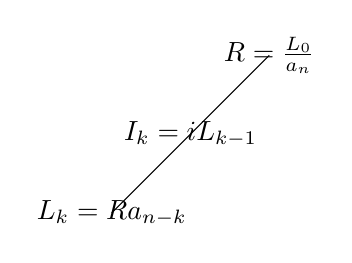
\begin{tikzpicture}
\draw (1,1) node{$L_k=Ra_{\angles{n-k}}$} -- (2,2) node{$I_k=iL_{k-1}$}-- (3,3) node{$R=\frac{L_0}{a_{\angles{n}}}$};
\end{tikzpicture}
\begin{exercise}
贷款一笔钱,n年内等额分期付款,每年末还一次,偿还金额是X,第一年利息是604RMB,第三年是593.75,第五年利息是582.45,计算X
\end{exercise}
\begin{note}
支付的利息:$I_k=iL_{k-1}=iRa_{\angles{n-k+1}}=R(1-v^{n-k+1})$
\end{note}
\begin{exercise}
按年实际利率i偿还一笔 1000 元的贷款。已知:\\
(1)在第6年末偿还第一笔款项\\
(2)然后每年未等额偿还一次在第15年末可以偿清这笔贷款(即一共偿还 10 次)\\
(3)在第10年末的付款结束后。未偿还本金余额为 908.91 元\\
试计算第5年末的未偿还本金余额
\end{exercise}
\begin{solution}
设等额付款金额为 $R: Ra_{\angles{5}i}=908.81, Ra_{\angles{10}}=1000(1+i)^5 \\
故第5年末的未归还本金为 $1000 \times(1+i)^{5}=1510.6$ 元
\end{solution}
\section{等额偿债基金}
区别:偿还本金采用不同的计息方式\\
$$D=\frac{L_0}{s_{\angles{n}j}}$$\\
$$R=I+D$$\\
$$L_k=L_0-Ds_{\angles{n}j}$$